

\tikzset{every picture/.style={line width=0.75pt}} %set default line width to 0.75pt        

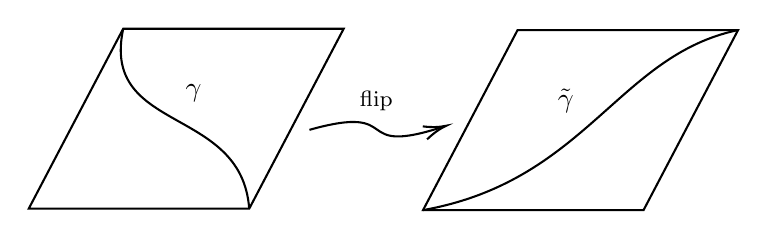
\begin{tikzpicture}[x=0.75pt,y=0.75pt,yscale=-1,xscale=1]
%uncomment if require: \path (0,342); %set diagram left start at 0, and has height of 342

%Shape: Parallelogram [id:dp9440132437357889] 
\draw   (106.2,82.67) -- (212.43,82.67) -- (166.9,169.39) -- (60.67,169.39) -- cycle ;
%Shape: Parallelogram [id:dp4450674539847944] 
\draw   (296.2,83.33) -- (402.43,83.33) -- (356.9,170.06) -- (250.67,170.06) -- cycle ;
%Curve Lines [id:da015686636387745367] 
\draw    (106.2,82.67) .. controls (95.28,133.39) and (163.28,119.39) .. (166.9,169.39) ;
%Curve Lines [id:da5146201674257586] 
\draw    (250.67,170.06) .. controls (329.28,156.06) and (344.61,95.39) .. (402.43,83.33) ;
%Curve Lines [id:da8815901966148098] 
\draw    (195.94,131.39) .. controls (242.8,118.19) and (214.52,144.85) .. (260.53,129.86) ;
\draw [shift={(261.94,129.39)}, rotate = 161.57] [color={rgb, 255:red, 0; green, 0; blue, 0 }  ][line width=0.75]    (10.93,-3.29) .. controls (6.95,-1.4) and (3.31,-0.3) .. (0,0) .. controls (3.31,0.3) and (6.95,1.4) .. (10.93,3.29)   ;

% Text Node
\draw (134.78,108.07) node [anchor=north west][inner sep=0.75pt]    {$\gamma $};
% Text Node
\draw (314.11,110.07) node [anchor=north west][inner sep=0.75pt]    {$\tilde{\gamma }$};
% Text Node
\draw (218.78,111.33) node [anchor=north west][inner sep=0.75pt]   [align=left] {{\footnotesize flip}};


\end{tikzpicture}
